\rhead{引言}
\chapter{引言}
%@@@@@@@@@@@@@@@@@@@@@@@@@@@@@@@@@@@@@@@@@@@@@@
\section{研究背景及意义}
蛋白质是分子生物学中具有极其重要意义的生物结构,因为它能更好的帮助我们理解细胞作用的机理,对于蛋白质序列的分析以及对于不同蛋白质之间进行序列匹配分析,都能很好的帮助我们理解蛋白质的功能及作用。

但是,蛋白质并不是单一活动的,往往一种生物的某个细胞活动,是需要许多蛋白质在一起相互作用,才能够完成的,而并不是靠某个单一的蛋白质就能完成了。因此就引出了生物学中的蛋白质相互作用网络这一模型(protein-protein interaction networks)。在以前,只是单纯通过比较两个蛋白质序列来确定蛋白质之间的相似程度。在有了PPI网络这一模型后,可以通过对不同的PPI网络之间的对比,来更精确的衡量不同蛋白质之间的相似程度。在一个PPI网络中,可以认为,一个蛋白质不单单表现为蛋白质序列,更表现为它与网络中其中蛋白质之间的相互作用,因此,当我们对比两个蛋白质时,应该将网络的相互作用考虑进去。

网络匹配(network alignment,NA)是指将两个不同物种的PPI网络进行匹配的过程。NA的目的在于找到两个PPI网络中极为相似的一些区域。因此,精准的网络匹配,对于分析在进化过程中处于近亲关系的物种之间的蛋白质作用,具有极为重要的意义。有了网络匹配,我们可以将一种生物的蛋白质作用过程,映射到另一生物的蛋白质网络中,那么后者的生物意义可以极大程度上参考前者。

而现在,大量的PPI网络数据与日俱增\cite{breitkreutz2008biogrid,hulovatyy2014revealing},这就要求更快,更好的网络匹配算法。因为从生物学角度来讲,想要通过生物学实验而一步步确定一个蛋白质的作用是非常缓慢的。而从生物信息学的角度来看,如果我们能够通过一个好的网络匹配算法,将已知生物网络和未知生物网络进行匹配,那么对于已知生物的许多生物学知识,便能够推广到未知生物当中去。因此,一个好的网络匹配算法具有极其重要的意义。

%@@@@@@@@@@@@@@@@@@@@@@@@@@@@@@@@@@@@@@@@@@@@@@@@@
\section{研究内容}
一个PPI网络可以看成是图论中的一个图(graph),其中,每个蛋白质由一个点(node)表示,而蛋白质与蛋白质之间的相互作用关系,则可以看成这个图中的边(edge),至于这个边是否带权重,则取决于问题。因此,网络匹配其实就是对两个图作匹配的过程,而目的则是尽可能找出两个图中相似的子结构。在图论中,寻找一个图在另一个图中的同构子图是一个NP完全的问题\cite{cook1971complexity}。因此,想要找到一个PPI网络在另外一个网络中的精确匹配是不可能的,我们只能期望达到尽量相似的结果。

从一般意义上来讲,网络匹配就是将两个网络的点进行匹配,使得所匹配的两部分子图,具有相似的结构特征,这个相似度,可以但从网络的拓扑结构上来考虑,也可以同时考虑蛋白质之间的序列相似性。

网络匹配,分为局部匹配(local network alignment,LNA),和全局匹配(global network alignment)。一开始,LNA是人们关注的重点,它的目的在于找到两个网络中局部高度匹配的区域(highly conserved),其产生的结果往往是两个网络中规模较小的子图,同时,一个网络中的点可能会匹配多个目标网络中的点。

\begin{figure}[htbp]
\centering
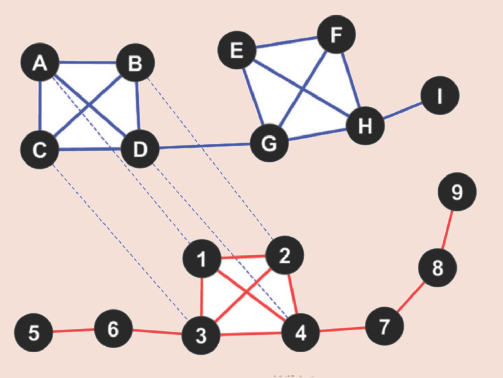
\includegraphics[height=0.25\textheight]{pic/lna.png}
\captionsetup{margin=50pt}
\caption{局部匹配,其中[1,2,3,4]可以和[A,B,C,D]匹配,也可以和[E,F,G,H]匹配 \cite{atias2012comparative} \label{fig:lna}}
\end{figure}
而全局匹配,顾名思义,则是从整体上来对一个网络进行匹配,它匹配的不是一个网络的子图,而是整个网络,并且,点与点之间的关系是一对一(one-to-one),而不是像LNA是多对多(many-to-many)。

\begin{figure}[htbp]
\centering
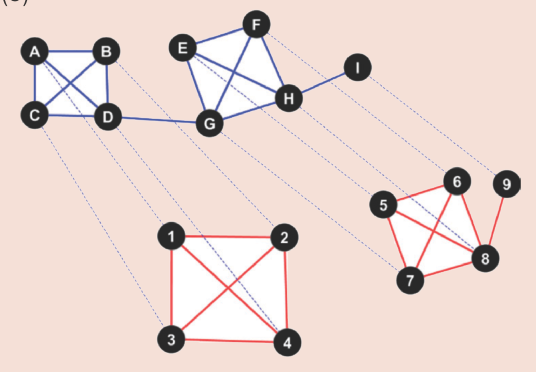
\includegraphics[height=0.25\textheight]{pic/gna.png}
\captionsetup{margin=50pt}
\caption{全局匹配,可以看到所有点都得到了匹配 \cite{atias2012comparative} \label{fig:gna}}
\end{figure}
相比于LNA注重两个网络中的局部相似性,GNA更关心一个网络在整体上和另一个网络的相似程度,而且近来越来越得到关注。

常见的局部网络匹配算法有PathBLAST\cite{kelley2004pathblast},NetworkBLAST\cite{sharan2005conserved},NetAlign\cite{liang2006netalign},MaWISh\cite{koyuturk2006pairwise}和Graemlin\cite{flannick2006graemlin}。之后,全局网络匹配算法被大量提出,常见的有IsoRank\cite{singh2008global,liao2009isorankn},GRAAL\cite{kuchaiev2011integrative,malod2015graal,kuchaiev2010topological,milenkovic2010optimal,memivsevic2012c},MAGNA和MAGNA++\cite{saraph2014magna,vijayan2015magna++},SPINAL\cite{aladaug2013spinal},PINALOG\cite{phan2012pinalog},Netcoffee\cite{hu2013netcoffee},BEAMS\cite{alkan2014beams}。而本文研究的重点也是全局网络匹配。

IsoRank\cite{singh2008global}可以说是全局匹配算法中的先驱,它定义了两个网络间任意点对之间的相似度分数(score),这个分数由这个两个点代表的蛋白质的结构信息(structural similarity)和序列信息(protein sequence similarity)同时决定。然后通过这个分数计算出最后得到的匹配结果。GRAAL一系列方法也定义了两个点之间的相似度,不过不同于IsoRank的是,GRAAL系列都通过衡量两个点之间的小图度数相似度(graphlet-degree)作为两个点之间的相似度分数。GRAAL\cite{kuchaiev2010topological}是这一系列方法中的第一个方法,它根据相似度分数,从高到低选择待匹配的点对,然后通过扩展这个点对的邻居来贪心的选择匹配点对。H-GRAAL\cite{milenkovic2010optimal}则用了二分图中的匈牙利算法来优化GRAAL中的扩展这一过程,使得产生的结果更好,而代价就是运行时间的增加。而MI-GRAAL\cite{kuchaiev2011integrative}则可以选择采用不同的相似度分数来进行点对匹配。L-GRAAL\cite{malod2015graal}则是GRAAL系列算法中最近提出来的算法,它将图匹配的问题建模成了一个线性规划的问题,然后从该问题中得到一个较优的解。SPINAL算法\cite{aladaug2013spinal}是一种迭代式算法,它通过不断扩展已匹配点周围的点来生成新的匹配点对。MAGNA\cite{saraph2014magna}则是运用了遗传算法来对已有匹配结果进行改进。

然而可以看到,到目前为止,所以已经提出的网络匹配算法,都是针对静态PPI网络的匹配,也就是说,待匹配的目标网络是单一不变的。而我们知道,生物细胞中的生命活动往往是动态的,而与细胞生命活动息息相关的蛋白质相互作用网络,其实是随时间变化的,可能在前一时刻两者还有相互作用的蛋白质,在后一时刻由于细胞生命活动的变更,而变得没有相互作用了。总体上来说,将生物体蛋白质之间的相互作用表达成一个静态的网络已经能够体现蛋白质之间的相互作用了,但是这种表示方式并不能体现时间维度上的特征。因此为了更好地匹配PPI网络,在动态PPI网络上作匹配是很有意义的。近来,有不少文章的工作是基于动态PPI网络的\cite{lin2010dynamic,chen2014identifying,wang2013construction}。而它们构造动态PPI网络的方式也不尽相同,而且研究的问题也不同。但是可以看到动态PPI网络正逐步受到人们的重视。

随之而来的问题就是,如何针对动态PPI网络,提出新的匹配算法呢?这也是本文要研究的内容。

本文首先提出了动态PPI网络的概念,然后提出动态PPI网络匹配的问题,最后提出相应的算法SGOPT,并用实验证明了该算法的效果。SGOPT是一种基于既有静态PPI网络匹配算法的,在动态PPI网络上优化匹配效果的算法,因此一般来说它可以和任意的既有静态PPI网络匹配算法结合。
%@@@@@@@@@@@@@@@@@@@@@@@@@@@@@@@@@@@@@@@@@@@@@@@@@@@@@@@@@@@
\section{本文结构}

第二章着重介绍了一些本文要研究的问题的相关概念,以及一些相关工作。第三章介绍了本文的主要贡献,包括动态PPI网络概念的定义,问题的定义,SGOPT算法的详细介绍等。第四章是实验分析部分。第五章总结文章。
